% to compile: Shift+Alt+F1
\documentclass[a4paper,11pt]{article}%,twocolumn
%% packages

\usepackage{blindtext} % needed for creating dummy text passages
%\usepackage{ngerman} % needed for German default language
\usepackage{amsmath} % needed for command eqref
\usepackage{amssymb} % needed for math fonts
\usepackage[colorlinks=true,breaklinks]{hyperref} % needed for creating hyperlinks in the document, the option colorlinks=true gets rid of the awful boxes, breaklinks breaks lonkg links (list of figures), and ngerman sets everything for german as default hyperlinks language
\usepackage[hyphenbreaks]{breakurl} % ben�tigt f�r das Brechen von URLs in Literaturreferenzen, hyphenbreaks auch bei links, die �ber eine Seite gehen (mit hyphenation).
\usepackage{xcolor}
\definecolor{c1}{rgb}{0,0,1} % blue
\definecolor{c2}{rgb}{0,0.3,0.9} % light blue
\definecolor{c3}{rgb}{0.3,0,0.9} % red blue
\hypersetup{
    linkcolor={c1}, % internal links
    citecolor={c2}, % citations
    urlcolor={c3} % external links/urls
}
%\usepackage{cite} % needed for cite
\usepackage[square,authoryear]{natbib} % needed for cite and abbrvnat bibliography style
\usepackage[nottoc]{tocbibind} % needed for displaying bibliography and other in the table of contents
\usepackage{graphicx} % needed for \includegraphics 
\usepackage{longtable} % needed for long tables over pages
\usepackage{bigstrut} % needed for the command \bigstrut
\usepackage{enumerate} % needed for some options in enumerate
%\usepackage{todonotes} % needed for todos
\usepackage{makeidx} % needed for creating an index
\makeindex
\usepackage{gensymb}
%\usepackage{url}
\usepackage{xurl}
\usepackage{psfrag}
\usepackage{multirow}
\usepackage{subfigure}

\usepackage{algpseudocode}
\usepackage{float}
%\usepackage{minted}
\usepackage{tcolorbox}
\usepackage{menukeys}
\usepackage[
width=.8\textwidth,
justification=centering]{caption}
\usepackage{xcolor}
\usepackage{pstricks}
\usepackage{acronym}
%% page settings

\usepackage[top=20mm, bottom=20mm,left=20mm,right=20mm]{geometry} % needed for page border settings
\parindent=0mm % for space of first line of new text block
\sloppy % for writing with hyphenless justification (tries to)
\hyphenation{} % use hyphenation of tolerance parametershttp://www.jr-x.de/publikationen/latex/tipps/zeilenumbruch.html
\hyphenpenalty=10000
\exhyphenpenalty=10000
\usepackage{fancyhdr} % needed for head and foot options
%% my macros

%% Text fomats
\newcommand{\tbi}[1]{\textbf{\textit{#1}}}

% IEEE naming convention
%\renewcommand{\figurename}{Fig.}

% custom counter for shell scripts
\newcounter{shellcounter}
% \newcounter{myexample}% preamble
\newtcolorbox[
use counter=shellcounter,
number format=\Alph]{shell}[2][]{%
	colback=blue!5!white,
	colframe=blue!75!white,
	fonttitle=\bfseries,
	title= {\sc Shell \thetcbcounter}: #2,#1}


\newcounter{outputcounter}
\newtcolorbox[
use counter=outputcounter,
number format=\Roman]{result}[2][]{%
	colback=green!5!white,
	colframe=green!75!black,
	fonttitle=\bfseries,
	title= {\sc Result box \thetcbcounter}: #2,#1}


\begin{document}
\begin{titlepage}
\center % Center everything on the page

%-------------------------------------------------------------------------------------
%	HEADING SECTIONS
%------------------------------------------------------------------------------------
\textbf{\large Department of Electronic and Telecommunication Engineering}\\[0.5cm]
\textbf{\Large University of Moratuwa, Sri Lanka}\\[1cm]
\textbf{\large EN4603 - Digital IC Design}\\[2cm]

\includegraphics[width=0.3\textwidth]{figures/uomlogo}\\[2cm]

	
%-------------------------------------------------------------------------------------
%	TITLE SECTION
%------------------------------------------------------------------------------------
\textbf{\Huge Laboratory Experiment 1 \\RTL Synthesis }\\[0.2cm]
\textbf{\Large Laboratory Report}\\[3cm]


%----------------------------------------------------------------------------------------
%	MEMBERS SECTION
%----------------------------------------------------------------------------------------


\vfill

\textbf{\large Submitted by}\\[0.5cm]

\textbf{\large Submitted by}\\[2mm]
\begin{minipage}{0.3\textwidth}
	\begin{flushleft}
		{\large C.S.Pallikkonda}\\[2mm]
		{\large R.M.A.S.Rathnayake }\\[2mm]
		{\large B.P.Thalagala }\\[2mm]		
		
	\end{flushleft}
\end{minipage}
\hspace{2mm}
\begin{minipage}{0.2\textwidth}
	\begin{flushright}
		{\large 180441C }\\[2mm]
		{\large 180534N }\\[2mm]
		{\large 180631J }\\[2mm]

	\end{flushright}
\end{minipage}\\[1cm]

	
	
	
%----------------------------------------------------------------------------------------
%	DATE SECTION
%----------------------------------------------------------------------------------------

\textbf{\large Submitted on}\\[0.5cm]
\textbf{\Large \today} % Date, change the \today to a set date if you want to be precise

%----------------------------------------------------------------------------------------

\vfill % Fill the rest of the page with whitespace

\end{titlepage}

\pagebreak

\tableofcontents
\vfill
\textit{\textbf{Note:}}\\
\textit{All the materials related to the report can also be found at \url{https://github.com/bimalka98/Digital-IC-Design}}

\pagebreak
\listoffigures
\listoftables
\section*{List of Abbreviations}
\addcontentsline{toc}{section}{List of Abbreviations}
\begin{acronym}
	\acro{asic}[ASIC]{Application Specific Integrated Circuit}
	\acro{atpg}[ATPG]{Automatic Test Pattern Generation}
	
	\acro{def}[DEF]{Design Exchange Format}
	\acro{dft}[DFT]{Design For Testability}
		
	\acro{gpdk}[GPDK]{Generic Process Design Kit}
		
	\acro{hdl}[HDL]{Hardware Description Language}
	
	\acro{ic}[IC]{Integrated Circuit}
		
	\acro{rtl}[RTL]{Register-Transfer Level}
	\acro{rx}[RX]{Receiver}
		
	\acro{tcl}[TCL]{Tool Command Language}
	\acro{tx}[TX]{Transmitter}
	
	\acro{uart}[UART]{Universal Asynchronous Receiver Transmitter}
	
\end{acronym}






\pagebreak
\section{Introduction}

\subsection{Practical}
In this practical, we will be using \textit{Cadence Genus - Ver. 18.10 } to perform \ac{dft} insertion into an example \ac{rtl} design, a \ac{uart} transceiver (shown in Figure \ref{fig:top_level}). As inputs to Genus, we will provide

\begin{enumerate}
	\item Source Verilog files
	\item Technology libraries provided by the fabrication plant (here, $45~nm$ educational \ac{gpdk} given by Cadence) : {\tt (.lib, .lef, .tch)}
	
	\begin{itemize}
		\item Library Timing (.lib) files specify timing (cell delay, cell transition time, setup and hold time requirement) and power characteristics of standard cells. Slow and fast libraries 	characterize standard cells with maximum and minimum signal delays, which could occur from process variations.

		\item Tch files are binary files that accurately characterize library elements, that include  capacitance and resistance.
		
		\item Library Exchange Format (LEF) specify design rules, metal capacitances, layer information…etc.
	\end{itemize}
	
	\item Timing constraints
\end{enumerate}

and will obtain the Scan-test compatible netlist (Verilog files), timing constrains (.sdc file), scan\ac{def} file and a set of files to be used as inputs to Cadence Modus for \ac{atpg} as output. We will then analyze, compare and comment on the area and ports of the design at various stages of the Scan test insertion design flow.

\begin{figure}[h]
	\centering
	\fbox{
		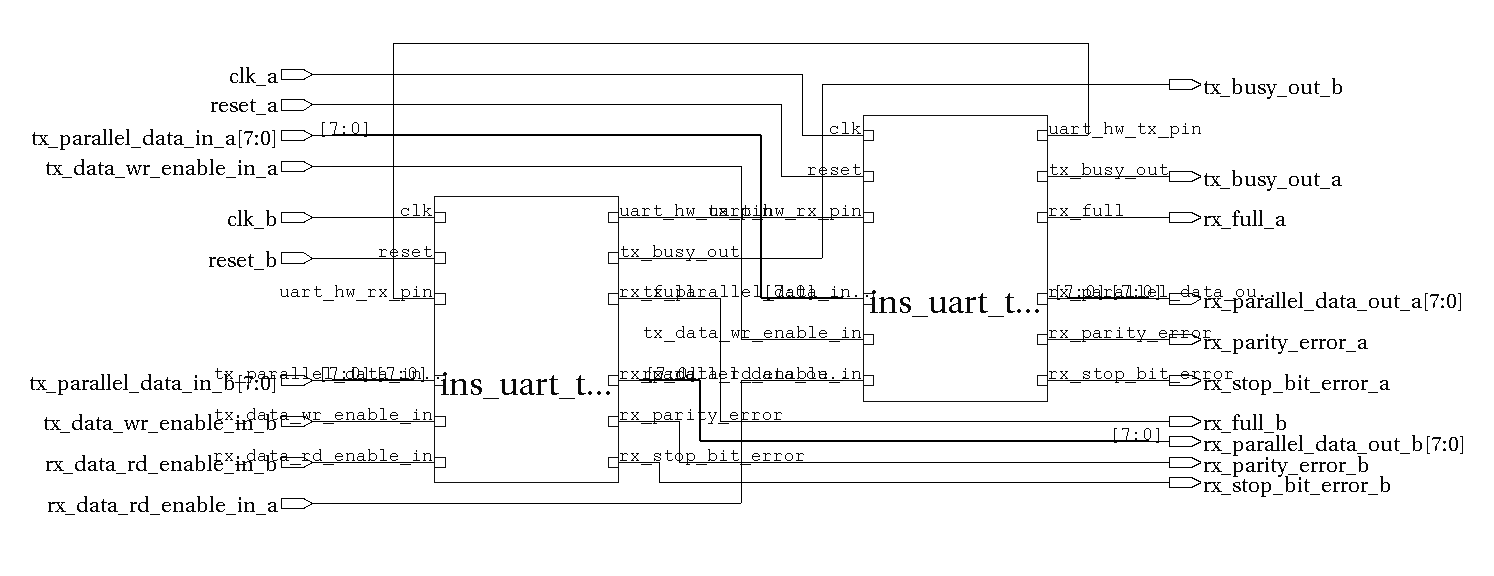
\includegraphics[width=0.95\linewidth]{figures/bw1.png}
	}
	\caption{Top level diagram of the \ac{uart} design}
	\label{fig:top_level}
\end{figure}

\pagebreak
\subsection{DFT Insertion}

In the context of \ac{asic} design, \ac{dft} refers to the process of inserting additional logic to improve the testability of the design. Here the testability is defined as the ability to communicate to the internal nodes through the primary input and output ports. The goal in \ac{dft} is to cover a maximum number of faults with a minimum amount of additional logic, as the insertion of additional logic directly translates to additional cost per chip.Although there are various \ac{dft} techniques in digital IC design, in this experiment, we will be focusing on inserting the `Scan Test' into an example design.


\begin{figure}[h]
	\centering
	\fbox{
		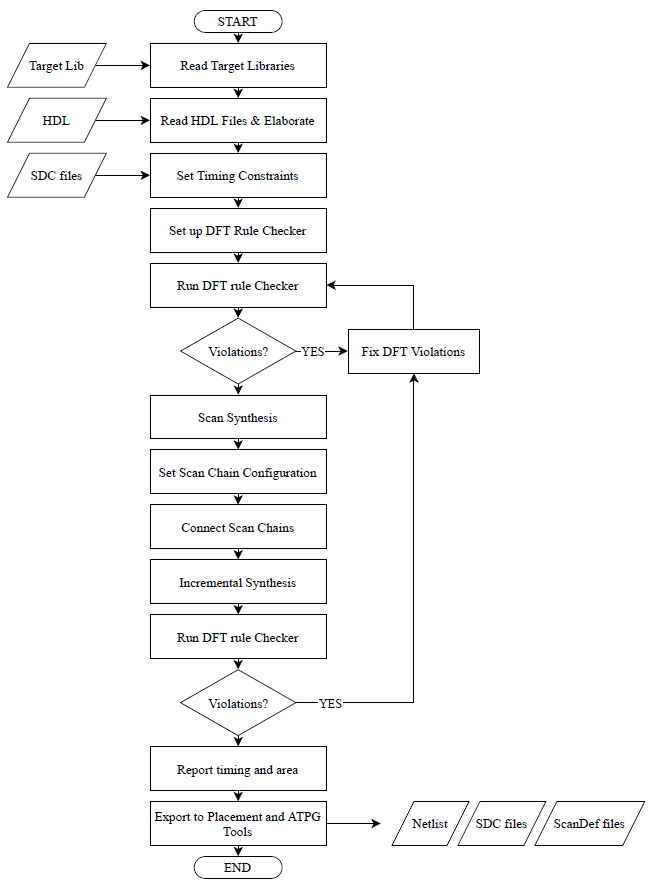
\includegraphics[width=0.8\linewidth]{figures/dftinsertion.png}
	}
	\caption{Overview of \ac{dft} insertion flow of 'Scan Test' in Cadence Genus software.}
	\label{fig:dftinsertion}
\end{figure}

\pagebreak
\subsection{Associated Genus Commands}

\textbf{Note}: \textit{Genus is a \ac{tcl} based tool and therefore {\tt .tcl} scripts can be created to execute a series of commands instead of typing each command individually. The entire interface of Genus is accessible through \ac{tcl}, and true \ac{tcl} syntax and semantics are supported.}\\

Followings are the commands used in this lab, and the entire script could be executed once using a single {\tt .tcl} file. However, it was encouraged to execute the commands one-by-one in order to understand the process of synthesizing an \ac{rtl} design.
\vspace{2cm}
\begin{Verbatim}[frame=single]
# 1. Link Technology Library
source ../scripts/setup.tcl

# 2. Read HDLs
read_hdl [glob ../input/rtl/*.v]

# 3. Elaborate the top module
elaborate uart_top

# Uniquify the top module
uniquify uart_top

# 5. Set timing constraints
source ../input/constraints.tcl

# Now that we have set the target libraries, 
# read the design files and set the design constrains,  
# we may now proceed to the DFT insertion steps.
# **************************************************************** 

# 7. Set the DFT scan style in order to configure the DFT rule checker
set_db dft_scan_style muxed_scan

# 8. Set the prefix for names of additional modules/ports
set_db dft_prefix dft_

# 9. Define shift_enable signal
define_shift_enable -name SE -active high -create_port SE

# 10. Run DFT rule checker
check_dft_rules

# If all steps have been followed correctly up until this point, 
# we should not see any DFT  violations
# ****************************************************************

# 11. Synthesize the design into the generic logic netlist,
# and then map to the technology library

# Synthesize to generic logic with medium effort
set_db syn_generic_effort medium
syn_generic

# Map to technology library and re-synthesize with medium effort
set_db syn_map_effort medium
syn_map

# 12. Write the scan synthesized netlist as uart_top_1.v
write_hdl > ../output/uart_top_1.v

# 13. Generate the reports after scan synthesis.
report_area > ../report/after_scan_synthesis/area.log
report_timing -nworst 10 > ../report/after_scan_synthesis/timing.log
report_port * > ../report/after_scan_synthesis/ports.log
report_power > ../report/after_scan_synthesis/power.log

# 14. Set scan configuration 
define_scan_chain -name top_chain_a -sdi scan_in_a -sdo scan_out_a
    -non_shared_output -create_ports -domain clk_a
define_scan_chain -name top_chain_b -sdi scan_in_b -sdo scan_out_b
    -non_shared_output -create_ports -domain clk_b

# 15. Preview the scan chains/Scan Stitching
connect_scan_chains -preview -auto_create_chains

# 16. Preview the scan chains/Scan Stitching
connect_scan_chains -auto_create_chains

# 17. Perform incremental synthesis to generate the netlist
# of the scan connected design
syn_opt -incr

# 18. Perform DFT rule check after scan connecting
check_dft_rules

# 19. Report scan setup and scan chain information
report_scan_setup > ../report/scan_setup.log
report_scan_chains > ../report/scan_chains.log

# 20. Write the DFT (scan test) inserted netlist and constrains.
write_hdl > ../output/uart_top_2.v
write_sdc > ../output/uart_top_2.sdc

# 21. Write the scanDEF file
write_scandef > ../output/uart_top_2_scanDEF.scandef

# 22. Generate the reports after scan connect
report_area > ../report/after_scan_connect/area.log
report_timing -nworst 10 > ../report/after_scan_connect/timing.log
report_port * > ../report/after_scan_connect/ports.log
report_power > ../report/after_scan_connect/power.log

# 23. Write the scripts required for the ATPG tool
write_dft_atpg -library
    ../input/libs/gsclib045/timing/slow_vdd1v0_basicCells.lib
\end{Verbatim}

\pagebreak
\section{Exercise}
This section documents the observations made in step 4 and 5 of the practical guide, with screenshots and explanations.\\


\vfill
\hrule
{\small
\bibliographystyle{IEEEtran}
\bibliography{refer}
}
%---------------------------------------------------------------------------
\end{document}
-
